\chapter{Design} \label{Design}

This chapter explores the design that will accomplish the goals delineated in Section \ref{sec:reserachgoal}. It first lays out the essential prerequisites that will help achieve the research goals. Moreover, in order to emphasize an accurate portrayal of upper limb rehabilitation, the chapter examines the requirements needed to correctly simulate a stroke movement and the frequency with which the FES is applied during the rehabilitation. 

These elements work together as guidelines for the design presented in the design overview. The design is highly inspired on paper \cite{QSC} therefore a comparison between the two projects is provided to help the reader understand the differences and similarities.

At the end of the chapter, the main tool Dynamic Arm Simulator (DAS) used for this project is explained in detail, including its main functionalities.


\section{Design Criteria} 

The project design must fulfil the following criteria to comply with all the research goals.

\begin{enumerate}
    \item \textbf{Real Arm Simulator with accurate dynamic representation} In order to correctly reproduce real-world dynamics and movements, an exact simulation of an arm was required a real arm simulator is needed. This arm simulator needs to behave and respond following the fundamentals of human biomechanics.
    \item \textbf{Tracking} Ability to track the arm´s movement either in joint space or task space. This will provide flexibility in the control system. 
    \item \textbf{EMG Reading} It should present the capability or a possibility to read real or fake muscle activity data. This data will be used as the main driven input to control the arm's stimulation.
    \item \textbf{Muscle Stimulation Control} There must be a way to actively control or access the muscle activity. This is important as the objective is to control the FES input based on EMG signals. 
    
\end{enumerate}

\section{Design Considerations: Stroke Coefficient and FES Frequency} \label{sec:design considerations}

When designing this project, two pivotal factors need to be meticulously considered: the simulation of stroke's effect on muscle activation and the optimal frequency for the FES system.

A stroke significantly alters muscle function. One of its notable manifestations is spasticity, a type of stiffness that depends on velocity. This condition commonly results in resistance to arm extension among stroke patients. Such effects are mainly due to increased activity in the biceps, wrist, and finger flexors, and a reduction in the activity of the triceps, anterior deltoid, wrist, and finger extensors \cite{IOL}. Taking into account these ramifications of stroke, this project primarily focuses on the triceps. Targeting this muscle is essential because stimulating it can augment muscle tone and reestablish motor control in affected muscles.

Regarding FES devices, their pulse frequencies typically span 23, 35, and 50 Hz \cite{NNPID}. For the purposes of this project, a frequency of 35 Hz has been selected.

\section{Design Overview}
The block diagram below (Figure \ref{fig:bdd}) shows an overview of the project design in relation to the objectives presented in Figure \ref{fig:researchgoals}.

\begin{figure}[h!]
    \centering
    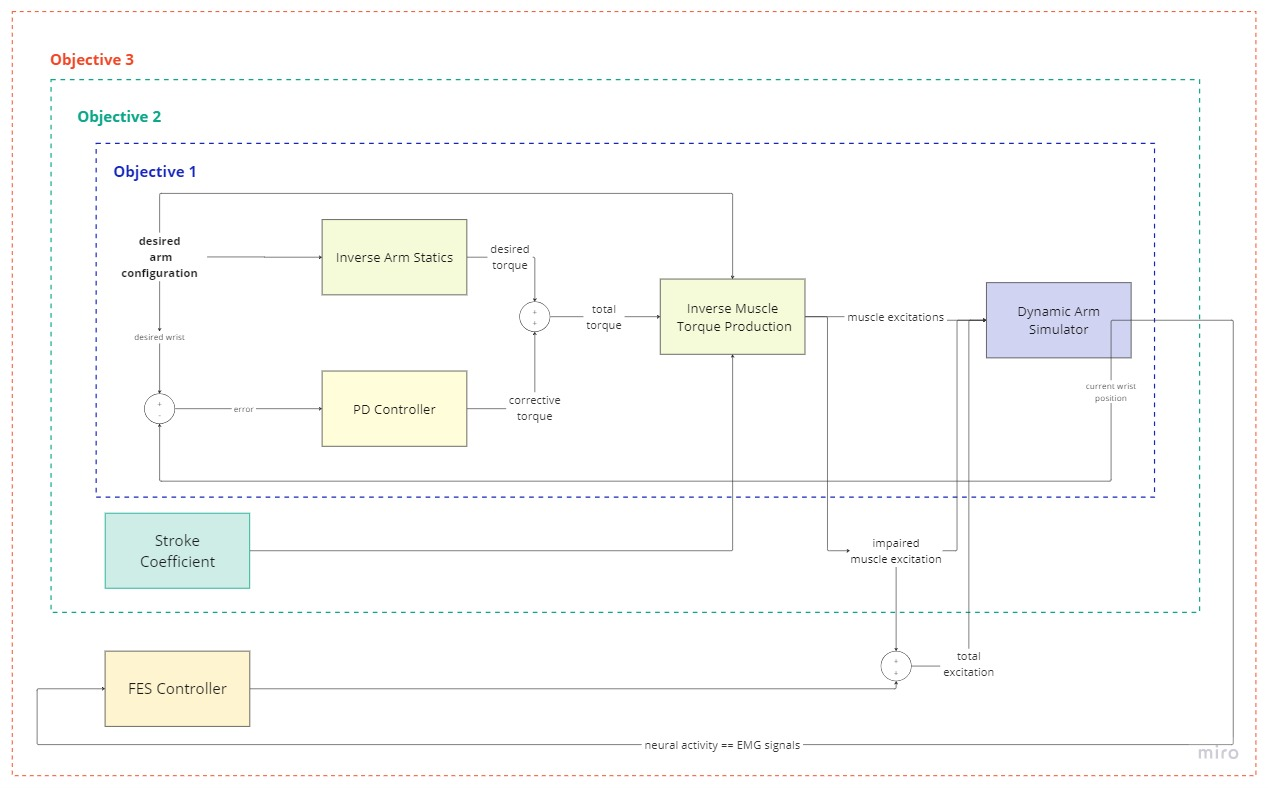
\includegraphics[width=\textwidth]{Pictures/blockDiagram.jpg}
    \caption{General Design Block Diagram}
    \label{fig:bdd}
\end{figure}

The first objective is to control the \ac{DAS} to achieve the desired arm configuration. To accomplish this, a quasi-static controller as inspired by the paper \cite{QSC} will be developed. Two models will be generated: the inverse arm statics, which correlates the arm configuration with the desired torque, and the inverse muscle torque production, which associates the torque with muscle excitation. This model will be the Gaussian Process Regression model as shown in \cite{QSC}. This muscle excitation mirrors the neural activation input to the \ac{DAS} responsible for executing the behaviour of the arm dynamics. Additionally, a PI controller is added to provide the corrective torque necessary to achieve the desired configuration. This torque will be added to the desired torque to produce the total torque which will then be again transformed into the corresponding muscle excitations. 

Upon successfully establishing a quasi-static controller for the simulated arm, a stroke coefficient will be introduced. This coefficient will modify the muscle excitations fed into the dynamic arm simulator. The adjustments will be grounded on research about the effects of stroke on arm motion, as detailed in Section \ref{sec:design considerations}. This will produce a compromised reaching motion often observed in stroke survivors.

Finally, a FES Controller will be designed to dynamically supplement the corresponding stimulation. This will ensure the manifestation of natural movement even when the individual exhibits stroke-induced motions.



\newpage
\section{Comparison between Simulation Studies}

Objective 1 is heavily influenced by the paper titled \textit{Developing a Quasi-Static Controller for Paralyzed Human Arm} (\cite{QSC}). The table below highlights the primary distinctions between this project and the aforementioned one for the readers better understanding. 

\setlength{\tabcolsep}{18pt}
\renewcommand{\arraystretch}{1.5}
\begin{table}[ht]
\caption{Comparison of Two Simulation Studies}
\label{tab:Comparison}
\resizebox{\textwidth}{!}{%
\begin{tabular}{|l|l|}
\hline
\multicolumn{1}{|c|}{\textbf{\begin{tabular}[c]{@{}c@{}}Developing a Quasi-Static Controller\\  for Paralyzed Human Arm\end{tabular}}} &
  \multicolumn{1}{c|}{\textbf{\begin{tabular}[c]{@{}c@{}}Developing an EMG-Based Quasi-Static\\  Controller for Stroke Reaching Rehabilitation\end{tabular}}} \\ \hline
Focused for spinal cord injury & Focused on stroke survivors                                                                             \\ \hline
Controlling 9 muscles          & Controlling 1 muscle                                                                                   \\ \hline
Surgical FES at 13Hz           & External FES stimulation at 30Hz                                                                               \\ \hline
Exoskeleton Arm Support        & \begin{tabular}[c]{@{}l@{}}No Exoskeleton Arm\\  (enough mobility provided by the patient)\end{tabular} \\ \hline
Wrist Position Control         & EMG and Wrist Position Control                                                                          \\ \hline
Multiple movements in the workspace &
  \begin{tabular}[c]{@{}l@{}}Different target, same initial positions. \\ Repetition of movement for rehabilitation purposes.\end{tabular} \\ \hline
\end{tabular}%
}
\end{table}
